\chapter{Analyse des besoins et conception}
\section*{Introduction}
Ce chapitre a pour objectif de planifier la réalisation du projet. Nous commençons par analyser les différents besoins ainsi que l'architecture technique de notre projet. Nous terminons par une description des divers outils que nous avons utilisés tout au long du processus de mise en œuvre de notre solution.
\section{Spécification des besoins}
Dans cette partie, nous nous concentrons sur la spécification des besoins pour guider la création du projet et déterminer les attentes de l'entreprise afin de clarifier les objectifs. Nous distinguons deux types de besoins, es besoins fonctionnels qui expriment les tâches que le système doit effectuer en réponse à une demande et les besoins non fonctionnels qui expriment les exigences implicites que le système doit avoir.

\subsection{Besoins fonctionnels}
Les besoins fonctionnels se diffèrent selon les exigences spécifiques d’une entreprise ou d’un projet. nous décrivons alors les besoins fonctionnels requis pour notre solution :
\begin{itemize}
    \item \textbf{Passage des appels via Asterisk} :
    Permettre la réalisation d'appels entre les membres de l'équipe via le serveur Asterisk à implémenter, en garantissant une qualité de service optimale pour les communications critiques.

    \item \textbf{Intégration avec la base de données interne} :
    Intégrer le serveur Asterisk avec une base de données MySQL propre à l'entreprise pour stocker les informations des utilisateurs, facilitant ainsi la gestion et l'analyse des données.

    \item \textbf{Automatisation de l'approvisionnement} :
    Utiliser Terraform comme outil d'infrastructure en tant que code (IaC) pour automatiser l'allocation des ressources nécessaires sur le cloud AWS, incluant les instances EC2 et le service de stockage de conteneurs ECR.

    \item \textbf{Dockerisation des serveurs Asterisk et MySQL} :
    Construire et conteneriser les images Docker pour les serveurs Asterisk et MySQL, assurant ainsi une portabilité et une facilité de déploiement dans différents environnements.

    \item \textbf{Stockage des images Docker} :
    Stocker les images Docker dans un service de stockage sur un cloud public, tel que le registre de conteneurs ECR d'AWS, pour une gestion centralisée et sécurisée des images.

    \item \textbf{Gestion de versions du code} :
    Gérer les branches et les versions du code source en utilisant Git, facilitant ainsi la collaboration entre les développeurs et le suivi des modifications du code.

    \item \textbf{Intégration continue} :
    Implémenter un pipeline CI avec GitHub Actions pour automatiser la construction des images Docker à chaque modification du code source, garantissant ainsi une livraison continue des nouvelles fonctionnalités et correctifs.

    \item \textbf{Déploiement continu} :
    Utiliser GitHub Actions pour automatiser le déploiement continu du serveur Asterisk sur le cloud, en déployant les images Docker stockées dans ECR sur les instances EC2, assurant ainsi une mise à jour rapide et fiable de l'environnement de pré-production.

    \item \textbf{Application cliente SIP} :
    Configurer et personnaliser une application cliente SIP open-source, comme Linphone, pour permettre aux utilisateurs de se connecter au serveur Asterisk et de tester les fonctionnalités d'appel.

        \item \textbf{Sécurité} :
    Assurer la sécurité des données, en mettant en place des mesures de protection adéquates pour le serveur Asterisk et la base de données MySQL.
    
    \item \textbf{Disponibilité} :
    Garantir une haute disponibilité du serveur Asterisk pour les utilisateurs.
\end{itemize}

\subsection{Besoins non fonctionneles}
En plus des besoins fonctionnels, nous spécifions les besoins non fonctionnels requis pour notre solution :

\begin{itemize}


    \item \textbf{Évolutivité} :
    Permettre une montée en charge facile du système en cas d'augmentation du nombre d'utilisateurs ou du volume de communications, en utilisant des solutions cloud pour ajuster les ressources en fonction des besoins.

    \item \textbf{Coût} :
    Réduire les coûts de fonctionnement par rapport à l'utilisation de l'application "StreamWide Team On Mission", en utilisant des solutions open-source et cloud pour maîtriser les dépenses.

    \item \textbf{Maintenabilité} :
    Faciliter la maintenance et les mises à jour du système grâce à l'utilisation de conteneurs et d'un pipeline CI/CD, et assurer une documentation complète et claire du processus de déploiement et de gestion du serveur.
\end{itemize}

\section{Architecture technique du projet}
L’utilisation d’une infrastructure en tant que code (IaC) permet d’allouer des ressources sur AWS et d’automatiser la création de notre propre infrastructure de déploiement. Cette automatisation s’appuie sur Terraform, un outil d’IaC, pour provisionner et gérer les ressources nécessaires de manière efficace et reproductible.\\
Pour connecter à notre cloud public, Il nous faut un compte
IAM (Identity and Access Management). Suite à l’exécution du code via la commande Terraform Apply, les ressources cloud seront créées. Ces derniers sont un registre des conteneurs (ECR), un réseau virtuel privé (VPC) avec un subnet public et un internet getway, un groupe de sécurité qui définit les règles d’accès à notre instance ubuntu EC2, un table de routage et son association avec le subnet créé, un générateur de clé privée et un générateur de clé public. La clé privée générée au sein de l’instance EC2 doit être copiée dans la machine locale pour connecter à l’instance via SSH. Dès que notre instance est lancée, un script bash sera executé pour y installer Docker et Git.\\ D'autre part, GitHub Actions se charge de déclencher le pipeline CI/CD suite à la détection d'un changement du code sur le répertoire Git. Ce pipeline assure la construction de notre serveur Asterisk et automatise son déploiement sur l'instance ubuntu. \\Donc, il se compose de deux phases, la première phase sert à créer une image Docker d'Asterisk en utilisant un Dockerfile la stocker dans ECR via la commande Docker Push. La deuxième phase c'est le déploiement de l'application sur AWS. L'image Docker stockée dans ECR sera copiée en local via la commande Docker Pull et lancée avec un serveur de base de données MySQL sur l'instance cloud en utilisant Docker-Compose, favorisant que les deux services fonctionnent respectivement sur les ports 5060 et 3306.\\ Après le déploiement, nous pouvons tester et effectuer des appels avec Linphone en tapant le nom de domaine IP du serveur Asterisk, le nom d'utilisateur et le mot de passe. La figure \ref{fig:archi_glob} illustre l'architecture technique de notre solution.
\begin{figure}[H]
        \centering
       \frame{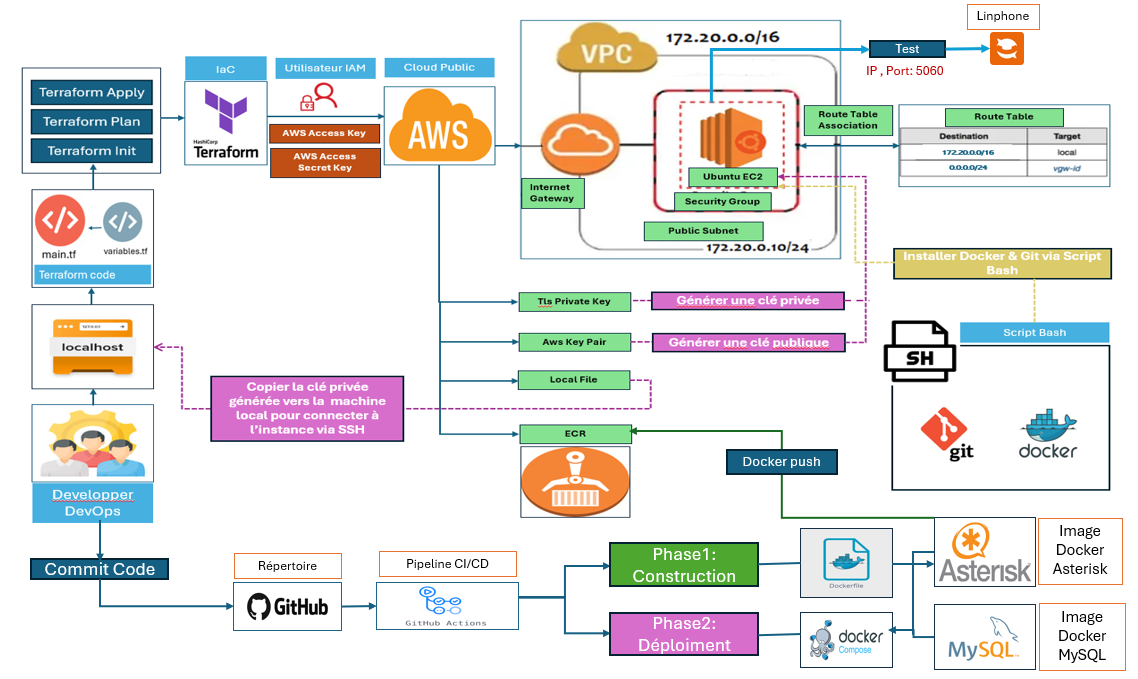
\includegraphics[width=17cm, height=14cm]{img/archi_détaillée.PNG}}
        \caption{Architecture technique du projet.}
        \label{fig:archi_glob}
\end{figure}

\section{Environnement de travail}
Durant cette partie, nous présentons les outils matériels et logiciels de notre projet. 

\subsection{Environnement de travail matériel}
L'ordinateur portable utilisé pour réaliser notre projet présente les caractéristiques suivantes :
\begin{itemize}
\item {Système d’exploitation : Windows 11 Pro}
\item {Processeur :  Intel Core i7-8565U, 4.6 GHz} 
\item {Mémoire installé (RAM): 16 Go}
\item {Disque dur : 1 To}
\end{itemize}

\subsection{Environnement de travail logiciel}
Avant de passer à la réalisation, nous identifions les technologies utilisées durant ce projet.

\subsubsection{Jira Software}
Jira Software présente un moyen de planification et de suivi des tâches d'un projet, développé par Atlassian. Il simplifie la collaboration et favorise l'agilité.

\subsubsection{Visual Studio Code}
Comme dans tout projet informatique, nous avons besoin d'un éditeur de code source comme Visual Studio Code. Ce logiciel développé par Microsoft est gratuit et open-source.

\subsubsection{Qt5}
Qt5 est un framework multiplateforme qui fournit des outils puissants pour la création d'interfaces utilisateur, la gestion des événements, et la communication inter-processus. En combinant Qt5 avec le langage C++, les développeurs peuvent créer des applications performantes et riches en fonctionnalités. Linphone notre application client est développée via cet outil.

\subsubsection{Docker}
Docker est un logiciel libre, utilisé pour créer des unités standardisées appelées conteneurs. Ces derniers sont utilisés pour isoler les applications de l’infrastructure afin de les déployer plus rapidement.

\subsubsection{Git}
Git est un outil de gestion des versions décentralisé, gratuit et open source, conçu pour une gestion rapide et efficace des projets.

\subsubsection{GitHub}
GitHub, est une platforme où les développeurs peuvent stocker, partager et gérer leurs fichiers Git. Au sein d’un dépôt Git, il est possible de stocker plusieurs versions d’une application, ce qui nous permet de contrôler les modifications apportées aux codes sources. Par le biais de GitHub Actions, fourni par GitHub, nous avons la possibilité de créer un pipeline CI/CD assurant l’automatisation des phases de construction et de déploiement.

\subsubsection{Terraform}
Terraform présente un outil d'infrastructure en tant que code IaC qui sert à automatiser notre infrastructure. Il fournit une solution d’automatisation simple et puissante pour la mise à jour des postes de travail et des serveurs, l'approvisionnement dans le cloud, la gestion de configuration, ainsi que l’orchestration des ressources.

\subsubsection{AWS}
AWS est une plateforme évolutive de Cloud Computing offrant des solutions complètes qui permettent aux entreprises d'accéder à des services et à des ressources informatiques moyennant l'Internet. Parmi les services utilisés, nous trouvons VPC, EC2 et ECR.

\section*{Conclusion}
Durant ce chapitre, nous avons tout d’abord analysé les besoins fonctionnels et non fonctionnels. Nous avons aussi détaillés l’architecture technique de la solution. Enfin, nous avons exposé l'écosystème matériel et logiciel du projet. Le chapitre suivant abordera la phase de réalisation.
